%\documentclass[en,hazy,blue,screen,14pt]{elegantnote}
\documentclass[en,hazy,blue,normal,12pt]{elegantnote}
\usepackage[T1]{fontenc}
\usepackage[latin9]{inputenc}
\usepackage{babel}
\usepackage{float}
\usepackage{textcomp}
\usepackage{amsmath,amsfonts,amssymb}
\usepackage{amsthm}
\usepackage{graphicx}
\usepackage[ruled,vlined]{algorithm2e}
\PassOptionsToPackage{normalem}{ulem}
\usepackage{ulem}
\usepackage{mathtools}
\usepackage{url}
\usepackage{hyperref}

\DeclarePairedDelimiter{\ceil}{\lceil}{\rceil}
\newcommand\tab[1][1cm]{\hspace*{#1}}
\newenvironment{claim}[1]{\par\noindent\underline{Claim:}\space#1}{}
\newenvironment{claimproof}[1]{\par\noindent\underline{Proof:}\space#1}{\hfill $\blacksquare$}

\title{Class Notes\\CIS 502 Analysis of Algorithm\\3-Graph Traversal}
\author{Da Kuang}
\institute{University of Pennsylvania}

\date{}

\begin{document}

\maketitle
\newpage
\tableofcontents
\newpage

\section{Graphics Basics}
\begin{itemize}
\item A graph G is an ordered pair of two sets $(V, E)$.
\item $V$ is a set of vertices/points/nodes, which is always a finite set.
\item $E$ is a set of unordered pair of vertices.
\item An edge is represented as $(u ,v)$. Here we abuse the notion of ordered pair to represent unordered pair.
\end{itemize}
% \centerline{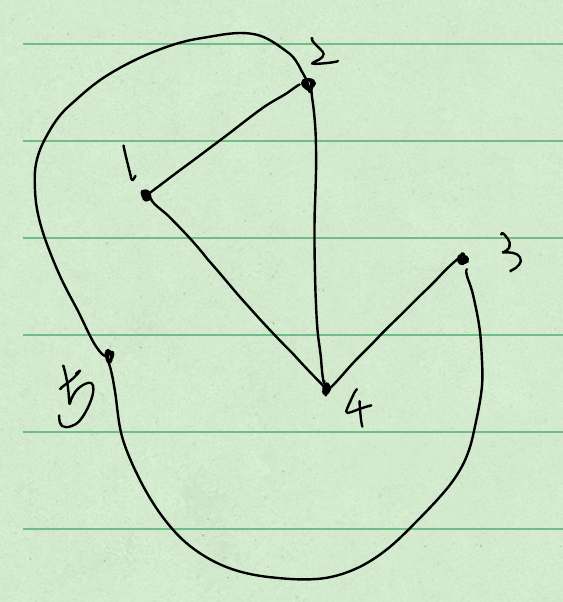
\includegraphics[width=0.2\textwidth]{graph.png}}

\subsection{Two representation of Graph}
When we talk about graph without adjective, that means it is a 
undirected graph. Suppose the number of vertices is $|V| = n$.
\begin{itemize}
 \item A vertex is incident to an edge if the vertex is one of the two vertices 
the edge connects.
\item If an edge $(u, v)$ has end points $u$ and $v$, we say it is an incident 
to vertex $u$ and $v$.
\item $u$, $v$ are adjacent if $(u, v) \in \mathbb{E}$.
\item The degree of vertex $v$ is the number of edges incident on $v$.
\end{itemize}

\subsubsection{Adjacency Matrix}
Adjacency Matrix is an symmetric matrix for undirected graph where
\[
V_{ij} = 
\begin{cases*}
 |(i,j)| & ,\text{ if $(i,j) \in \mathbb{E}$.}\\
 0  &,\text{ otherwise.}
\end{cases*}
\]

Space = $O(n^2)$.
\subsubsection{Adjacency List}
Adjacency List is an array of size $n$ of linked list, where $i$-th entry is 
a linked list consisting of the neighbors of vertex-$i$. It is default  representation of graph.

Space = $O(n + m)$.
\newpage
\subsection{Connectivity}
\subsubsection{Path}
A path in a graph is a sequence of vertices
\[v_0 v_1 \cdots v_k\]
, such that $(v_i, v_{i+1}) \in \mathbb{E}$ for $i = 0, 1, 2, \cdots, k-1$.

A simple path is a path that does not repeat vertices.
\paragraph{Lemma:}
If there is a path $(u, v)$, there must be a simple path $(u, v)$.
\subsubsection{Cycle}
A cycle in a graph is a sequence of vertices
\[v_0 v_1 \cdots v_kv_0\]
, such that $(v_i, v_{i+1}) \in \mathbb{E}$ for $i = 0, 1, 2, \cdots, k-1$ and 
$(v_k, v_{0}) \in \mathbb{E}$. All $v_i$'s are distinct.

\subsubsection{Connectivity}
\begin{itemize}
 \item $u$, $v$ is \textbf{connected} if there is a path between them.
 \item $G$ is \textbf{connected} if $\forall u, v \in V$, there is a path 
between $u$ and $v$.
\item The \textbf{connected components} of $G$ are maximal subset of vertices 
that are pairwise connected.
\end{itemize}

\subsubsection{Connection is equivalence relation}
Connection relation in a graph is an equivalence relation.
\begin{itemize}
 \item Reflexive Relation (take Path of length 0)
 \item Symmetric Relation (reversible path)
 \item Transitive Relation: If a Graph has a $uv$ path and also $vw$ path then 
it will also contain $uw$ path.
\end{itemize}
Because connection is the equivalence relation, pairwise connected vertices 
form a connected component.

\section{Tree}

Tree is a connected acyclic graph.
\subsection{Rooted tree}
\subsubsection{Inductive Definition}
A nice thing about Inductive definition is it is useful for the proofs by 
induction.
\begin{itemize}
 \item \textbf{Rule 1:} A graph consist of a single vertex v is a rooted tree 
with v as the root.
 \item \textbf{Rule 2:} If $(T_1, r_1)$, $(T_2, r_2), \cdot, (T_k, r_k)$ are 
rooted trees, then the tree $(T, r)$ consisting of a new node $r$ as root and 
edges $(r, r_1), \cdots, (r, r_k)$ is a rooted tree.
\end{itemize}
\subsection{Structural induction Proof}
Statement: Any tree with $n$ nodes has $n-1$ edges.

Since any tree can be transformed into a rooted tree, the induction can be as 
following:
\begin{itemize}
 \item Statement: Any rooted tree on $n$ nodes has $n-1$ edges.
 \item Base case: Single node tree with no edge. The statement is true.
 \item Inductive hypothesis: For a rooted tree $T_r$, built up from $(T_1, 
r_1), (T_2, r_2), \cdots, (T_n, r_n)$ using rule 2. Assume the statement is 
true for all the trees $T_1, T_2, \cdots, T_k$ and prove it for $T$.
\item Inductive step:
    \begin{itemize}
    \item Let tree $T_i$ have $n_i$ nodes, $i = 1, 2, \cdots, k$. Then $T$ has 
    $\sum_{i=1}^k n_i + 1$ nodes.
    \item By the inductive hypothesis, $T_i$ has $n_i - 1$ edges.
    \item Total number of edges is $T = \sum_{i=1}^k (n_i - 1) + k = 
\sum_{i=1}^k 
    n_i$.
    \item The number of edge is one less than the number of nodes. It proofs 
the     inductive step.
    \end{itemize}
 \end{itemize}

\paragraph{Remark:} Therefore, it takes $n-1$ comparisons to select the largest from $n$ numbers by tournament comparison.

\section{Traversal}

Traversal: Visiting all parts of the graph. Unlike linear data structures (Array, Linked List, Queues, Stacks, etc) which have only one logical way to traverse them, trees can be traversed in different ways. Following are the generally used ways for traversing trees.

\begin{figure}[H]
\centering
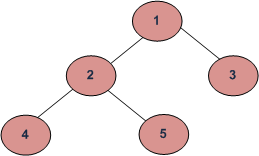
\includegraphics[width=0.3\textwidth]{tree12.png}
\end{figure}

\begin{itemize}
\item Depth First Traversals:
    \begin{itemize}
     \item Inorder (Left, Root, Right) : 4 2 5 1 3
     \item Preorder (Root, Left, Right) : 1 2 4 5 3
     \item Postorder (Left, Right, Root) : 4 5 2 3 1
    \end{itemize}
\item Breadth First or Level Order Traversal : 1 2 3 4 5

\end{itemize}

\subsection{Bread-first Search (BFS)}
Most of the cases, BFS is used to find out the shortest path from an unweighted 
and undirected graph.
\subsubsection{Basics}
\begin{itemize}
    \item Input:Graph $G = (V, E)$; a vertex $s$ as starting point.
    \item Goal: Visit all the vertices in systematic manner.
    \item Intuition: Think of the graph is drawn as a pond of water. Drop a 
stone at vertex v and watch the ripple expand with great regularity. The 
order of vertex visited in BFS is like the wave of ripples visiting the 
vertices.
\end{itemize}

\subsubsection{Algorithm}

\paragraph{3 possible states for each vertex:}
\begin{itemize}
 \item Undiscovered
 \item Discovered: Just find out this vertex and have not check its neighbors.
 \item Finished: discover the node and all its neighbors.
\end{itemize}
\paragraph{Queue:}
\begin{itemize}
 \item Initialized with just vertex $s$. $Q \leftarrow \{x\}$. x is discovered.
 \item Work the follows repeatedly:
 \begin{itemize}
  \item Pull a vertex out of the queue.
  \item Put all its neighbors into the queue as discovered.
 \end{itemize}
\end{itemize}

\paragraph{Example:}
An example of BFS starting from vertex $x$.
\begin{figure}[H]
\centering
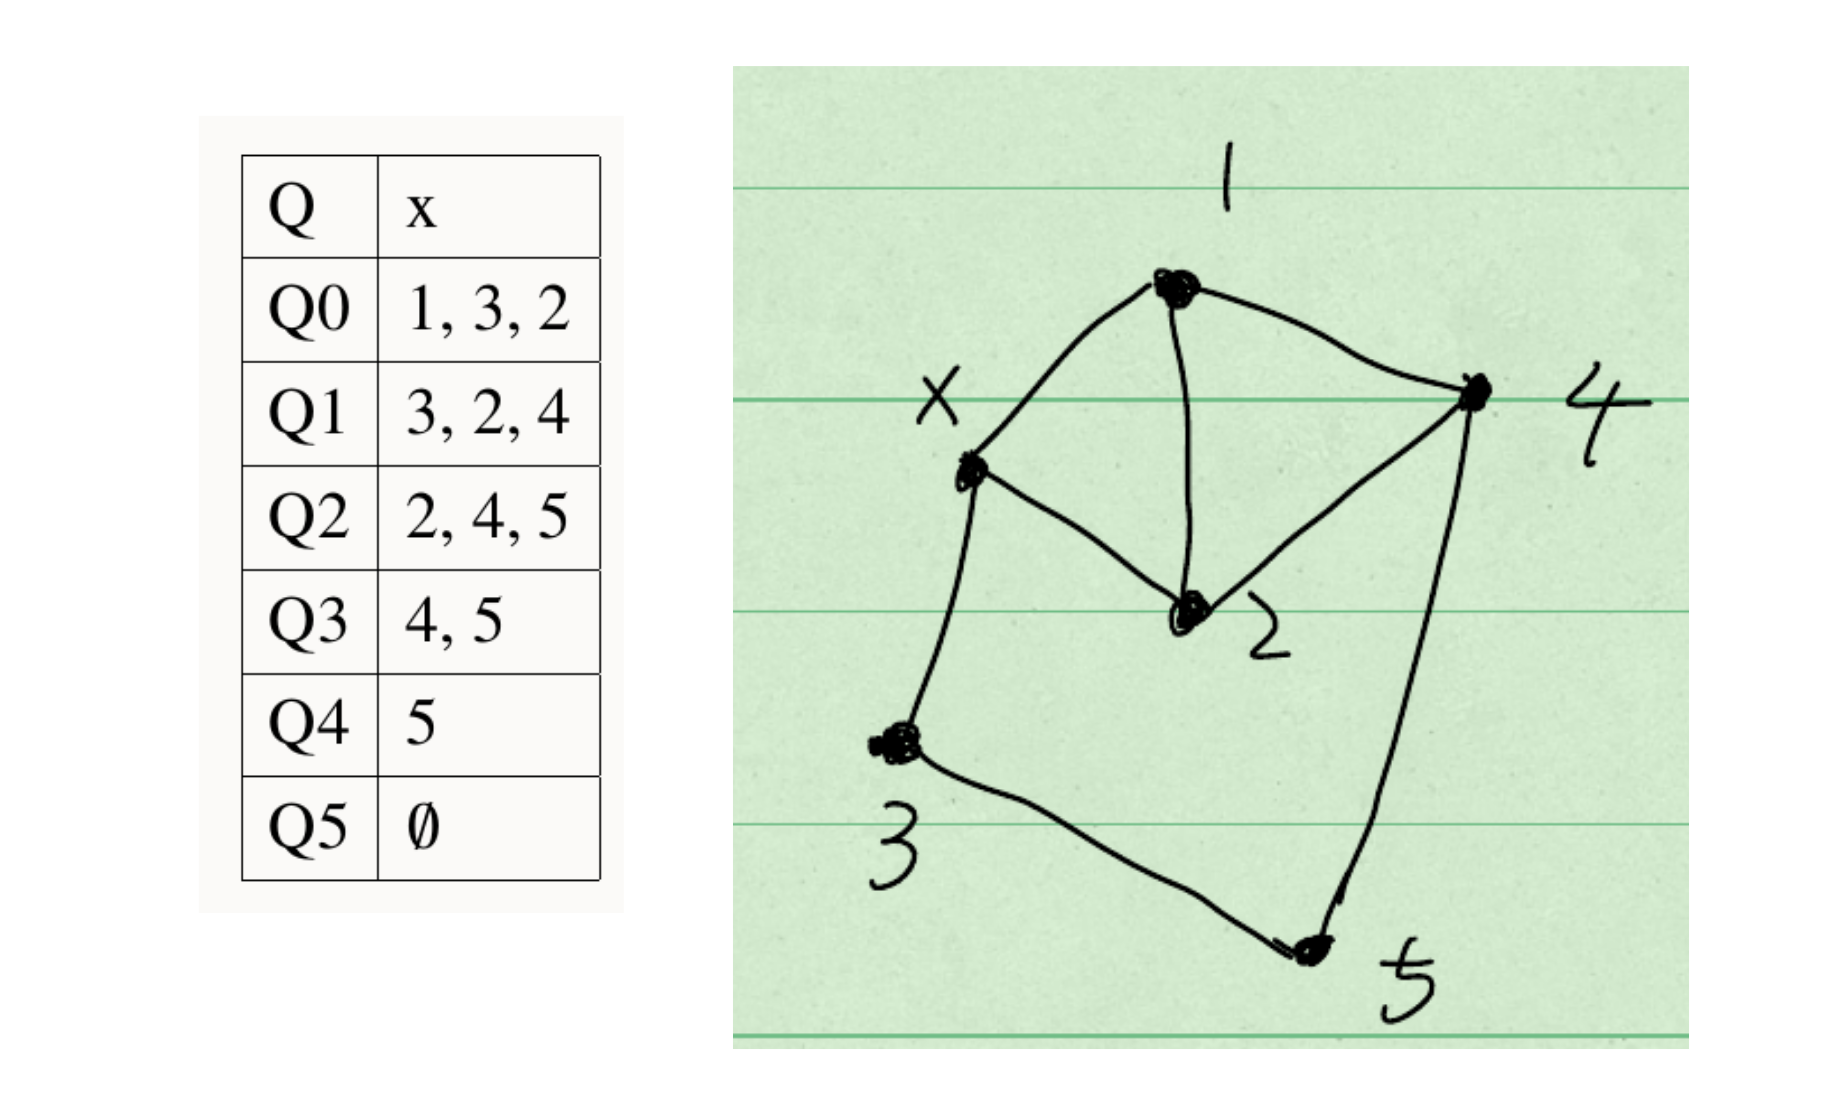
\includegraphics[width=0.5\textwidth]{queue.png}
\end{figure}

\paragraph{Remarks:}
\begin{itemize}
 \item In $Q1$, we did not put vertex $2$ into the queue since it is already in 
the Queue.
\item Vertices in queue are discovered.
\item Moving vertices out of the queue means it is finished.
\end{itemize}
\subsubsection{Levels}
\paragraph{Definition.}
Associate levels with vertices in BFS: 
\begin{itemize}
 \item The starting vertex is level 0: $\text{level}(s) = 0$.
 \item Any vertex $v$ is discovered when dequeue some vertex $u$, we set
\[\text{level}(v) = \text{level}(u) + 1\]
\end{itemize}

\begin{theorem}
 The level of $v$ is the smallest number of hops to get from $s$ to $v$.
\end{theorem}

\begin{proof}
 Let $\delta(s, v)$ be the smallest number of hops from $s$ to $v$. Prove that for any $v$, $\delta(s, v) = \text{level}(v)$.
\end{proof}

\begin{claim}
 $\delta(s, v) \le \text{level}(v)$.
\end{claim}

\begin{claimproof}
If $v$ has level $\text{level}(v)$, there is a sequence of vertices $$x, ~v_1, 
~v_2, ~\cdots, ~v_{\text{level}(v) - 1}, ~v$$, s.t. each one discovered from 
the previous.

We have shown one path from $x$ to $v$ which has $\text{level}(v)$ hops. 
Therefore, the smallest number of hops should be less or equal to the number of 
hops in this path. Therefore, $\delta(x, v) \le \text{level}(v)$.
\end{claimproof}
\begin{claim}
 $\delta(s, v) \ge \text{level}(v)$.
\end{claim}
\begin{claimproof}
Prove by contradiction. Suppose among all $v$ such that $\delta(s, v) < 
\text{level}(v)$, find the one with smallest $\delta(x, v)$.
\begin{figure}[H]
\centering
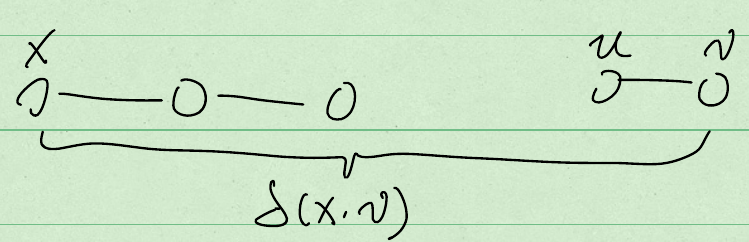
\includegraphics[width=0.5\textwidth]{level.png}
\end{figure}

Let $(s ~\cdots ~uv)$ be the path with fewest hops form $s$ to $v$.
\begin{align*}
&\delta(s, u) = \delta(s, v) - 1
\intertext{since $\delta(s, u) < \delta(s, v)$ and $\delta(s, v)$ is the 
smallest hops which less than level,}
\intertext{$\delta(s, u)$ must be larger than level$(u)$, i.e.}
&\text{level}(u) \le \delta(s, u) = \delta(s, v) - 1
\intertext{$v$ is the neighbor of $u$,}
&\text{level}(v) \le \text{level}(u) + 1 \le \delta(s, v)
\end{align*}
But we assume $\delta(s, v) < \text{level}(v)$, so we meet a contradiction the 
claim is true.
\paragraph{Notes}
\begin{itemize}
 \item $\text{level}(v) \le \text{level}(u) + 1$.\\
    Because $v$ can be discovered early than discovering from $u$.
\item Path $(s,v)$ is the shortest path which satisfies $\delta(s,v) < \text{level}(v)$. Therefore, any sub-path within $(s, v)$ has a $\delta$ greater than its level.
\end{itemize}
\end{claimproof}

\subsubsection{Remarks}
Look at edges on which new vertex are discovered. These edges from a tree and 
the discover sequence becomes the direction between vertices. Think 
of the tree are directed away from $s$, even though the graph is undirected.

Why it is a tree? Each vertex can be discovered at most one time. Every 
vertex at most have one in-coming edge then the graph is acyclic.

Will the tree contains all the vertices in the graph? 

No. The graph could have 
several isolated components. This is the expected result by design because BFS 
is used to find the shortest path from the source. So we do not want to find 
the vertex in different components because there is no path from the vertex to 
the source.

Will all the vertices in the same component with $s$ be discovered by BFS?
Prove by contradiction. There are some vertices in the component of $s$ that 
BFS starts which are not discovered. Among all such vertices, choose the one 
with the fewest hops away from the source.
% TODO: Prove it.
\subsection{Depth-first Search (DFS)}
The usage of DFS is broader than BFS. Explore one path as far as it will go, 
back track as little as needs. Repeat.

\subsubsection{Basics}

\paragraph{3 possible states for each vertex:}
\begin{itemize}
 \item Undiscovered
 \item Discovered: Just find out this vertex and have not check its neighbors.
 \item Finished: discover the node and all its neighbors.
\end{itemize}
\paragraph{Data Structure}
\begin{itemize}
\item BFS: Order of exploration of vertices is the same as the order of 
discovery. It is a FIFO, therefore we use queue to track discovered vertices.
\item DFS: Last discovered vertex is the first to be fully explored. It is a 
LIFO, therefore we use a stack to track the discovered vertices.
\end{itemize}
You get a stack for free by using recursion because during the recursion the 
OS maintains a stack by itself. Therefore, we can think about DFS as a 
recursive algorithm.

\subsubsection{Algorithm}
$DFS(G, s)$
\begin{itemize}
    \item Mark all vertices as undiscovered.
    \item Start with s and mark $s$ as discovered.
    \item While there is an undiscovered neighbor $u$ of $s$ call $DFS(G, u)$.
    \item Mark $s$ as finished.
\end{itemize}

\subsubsection{DFS Tree}
Formed by the set of edges on which new vertices are discovered. 

\begin{theorem}
In an undirected graph, if $(u, v)$ is an edge in the graph that is not in the DFS tree. Then $u$ is an ancestor of $v$ or $v$ is an ancestor of $u$ in the DFS tree.
\end{theorem}

\begin{proof}
% Should know the proof
Those edges are called ``back edges''. In an undirected graph you can only 
have tree edges and back edges.
\begin{figure}[H]
\centering
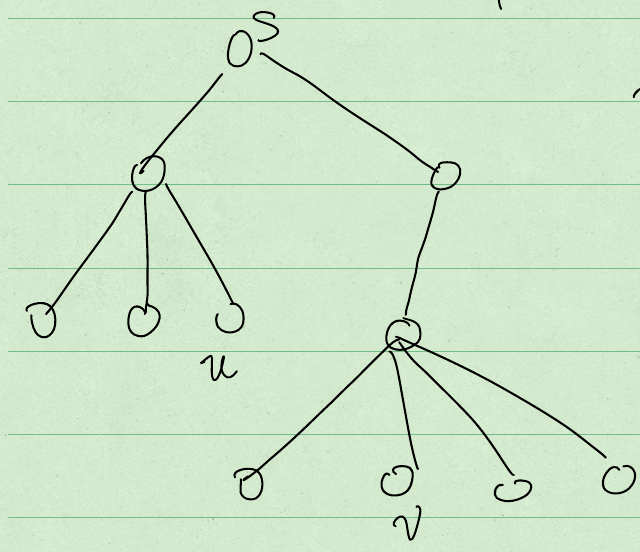
\includegraphics[width=0.5\textwidth]{dfs.png}
\end{figure}
This cannot exist because $v$ would have been discovered from $u$.
\end{proof}
\subsubsection{Time}
Suppose $u$ is a vertex in an undirected connected graph $G$.
\begin{itemize}
\item Time advance at each call and return of DFS function. The range of time 
is $[1, 2n]$.
\paragraph{Notes:} Every time you finish a recursive call of DFS, time advance 
by 1. Every time you make a new recursive call time advance by 1. Time is 
discrete and start from 1 at the first DFS call to $s$ and advance by 1 every 
time you finish or start a new recursive call.
\item $s(u)$: \textbf{The start time} of $u$ is the time at which DFS of $u$ is 
invoked.
\item $f(u)$: \textbf{The finish time} of $u$ is the time at which the DFS of 
$u$ is finished.
\end{itemize}
\subsubsection{Duration}
It is generally true for recursive function that the duration of an vertex $u$ 
is the integral from the start to the finish time.
\[\text{Duration}(u) = [s(u), f(u)]\]
$\forall u, v,$ it is not the case that 
\[s(u) < s(v) < f(u) < f(v)\]
Recursive algorithm ensures that it does not happen since it is last in first 
out. $v$ should finish first before $u$.

\subsubsection{Lineage}
\begin{itemize}
\item \textbf{Ancestor:} If you have a rooted tree, $u$ is call ancestor of 
$v$ if $u$ is on the path from $v$ to the root. 
\item \textbf{Descendant:} If $v$ is an ancestor of $u$, then $u$ is the 
descendant of $v$.
\item By convention, we include itself as ancestor so we allow $v$ to be its 
own ancestor as well as its own descendant.
\end{itemize}
\begin{theorem}
Suppose $u$ is discovered before $v$ and there is a path \textbf{of 
undiscovered vertices} between $u$ and $v$. Then $v$ will become a descendant 
of $u$.
\end{theorem}
\begin{proof}
Prove by contradiction. Suppose it is not the case and look at the first 
vertex on the path from u to v of undiscovered vertices that dose not become 
the descent of $u$.

Look at the first vertex to violate the rule would be a good way to prove a 
contradiction.
% TODO: prove this theorem
\end{proof}
\subsection{Notes}
BFS is used to find the shortest path from the source in the graph therefore we 
start BFS from the source until we exhaust the component where the source lies.

DFS is also used to get a global picture of the entire graph and we often want 
DFS to be deterministic enough. We start from the source and do DFS. We only 
discover the vertices in the connected component of that source. But we want to 
discover other vertices. So we have a outer layer to restart the DFS from some 
undiscovered vertices in some other component every time we finish the search 
within one component. In this way, DFS is able to cover all the vertices and 
all the components. Therefore, often you only need to give DFS a graph without 
any source explicitly.

Ideally, BFS and DFS are just different traversal strategies, so the total run time should be the same which is the number of nodes plus the number of edges. In practice, the running time depends on how to access the nodes and edges. By convention, assume $|V| = m$, $|E| = n$. If the graph is an adjacency matrix, the run time is $O(|m|^2)$. If the graph is an adjacency list, the run time is $O(|n| + |m|)$.

\section{Equivalence Relation}
\begin{itemize}
\item A relation $R$ on a set $A$ is an equivalence relation if it is 
reflexive, symmetric, and transitive.
\item When the elements of some set $A$ have a notion of equivalence defined on 
them, then one may naturally split the set $A$ into equivalence classes.
\item If $R$ is an equivalence relation on the set $A$, its equivalence classes 
form a partition of $A$.
\item In each equivalence class, all the elements are related and every element 
in $A$ belongs to one and only one equivalence class.
\item The relation $R$ determines the membership in each equivalence class, and 
every element in the equivalence class can be used to represent that equivalence 
class.
\item In a sense, if you know one member within an equivalence class, you also 
know all the other elements in the equivalence class because they are all 
related according to $R$.
\item Conversely, given a partition of $A$, we can use it to define 
an equivalence relation by declaring two elements to be related if they belong 
to the same component in the partition.
\end{itemize}
\begin{figure}[H]
\centering
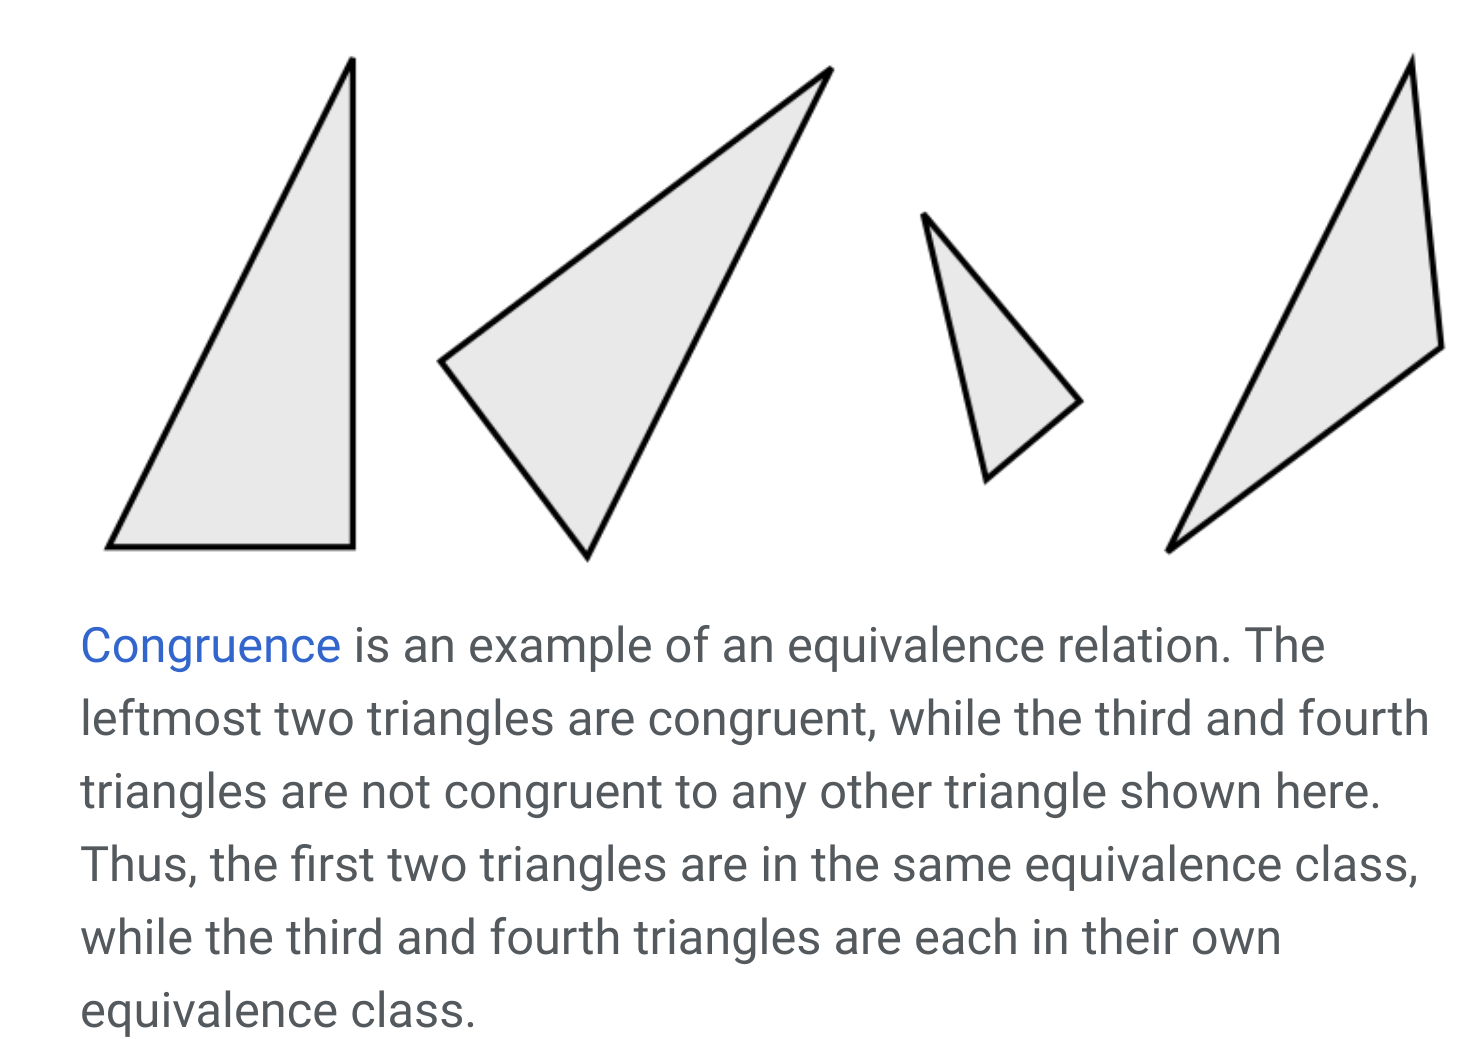
\includegraphics[width=0.5\textwidth]{equ-class.png}
\end{figure}
Ref: 
\begin{itemize}
\item \href{
https://math.libretexts.org/Courses/Monroe_Community_College/MTH_220_Discrete_Ma
th/6\%3A_Relations/6.3\%3A_Equivalence_Relations_and_Partitions}{equivalence}
\item \href{https://en.wikipedia.org/wiki/Equivalence_class}{Equivalence Class}
\end{itemize}

\section{Undirected Application: Bi-connectivity}

Connectivity is important but sometimes it is not enough and we want some 
robust connectivity. So we introduce \textbf{Bi-connectivity}.
\subsection{Definitions}
\subsubsection{Bi-connectivity}
\begin{itemize}
\item A graph is called biconnected if the removal of any one vertex leaves it 
connected.
\item A graph is called k-connected if the removal of any $k-1$ vertices leaves 
it connected.
\end{itemize}
Examples of connected graph which is not bi-connected.
\begin{figure}[H]
\centering
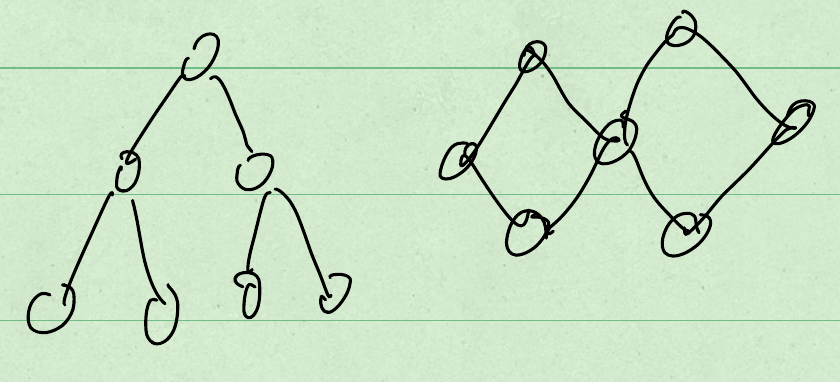
\includegraphics[width=0.5\textwidth]{bi-connectivity.png}
\end{figure}
\subsubsection{Articulation Point}
A vertex in an undirected connected graph is an \textbf{articulation point} (or 
cut vertex) \textbf{iff} removing it (and edges through it) disconnects the 
graph. 

Articulation points represent vulnerabilities in a connected 
network-single points whose failure would split the network into 2 or more 
disconnected components.

\subsubsection{Bi-connected Components}
Bi-connected Components are maximal pieces of the graph that are bi-connected.

\subsubsection{Vertex-disjoint Path}
Two paths are vertex-independent (alternatively, internally 
\textbf{vertex-disjoint}) if they do not have any internal vertex in common. 

Similarly, two paths are edge-independent (or edge-disjoint) if they do not 
have any internal edge in common. Two internally vertex-disjoint paths 
are edge-disjoint, but the converse is not necessarily true.

\subsubsection{Relations on edges}
How to define the relation between two vertices?

\paragraph{Proposal:} If there are two vertex-disjoint paths between $u$ and 
$v$, then $(u, v) \in R$. See example (a) in the following graph.

The proposal does not work because the relation is not Transitive. In other 
words, if $(u, v) \in R$ and $(v, w) \in R$ it is not always the case that 
$(u, w) \in R$.
See example (b) in the following graph. $(1, 6) \in R$ is a false statement.

\begin{figure}[H]
\centering
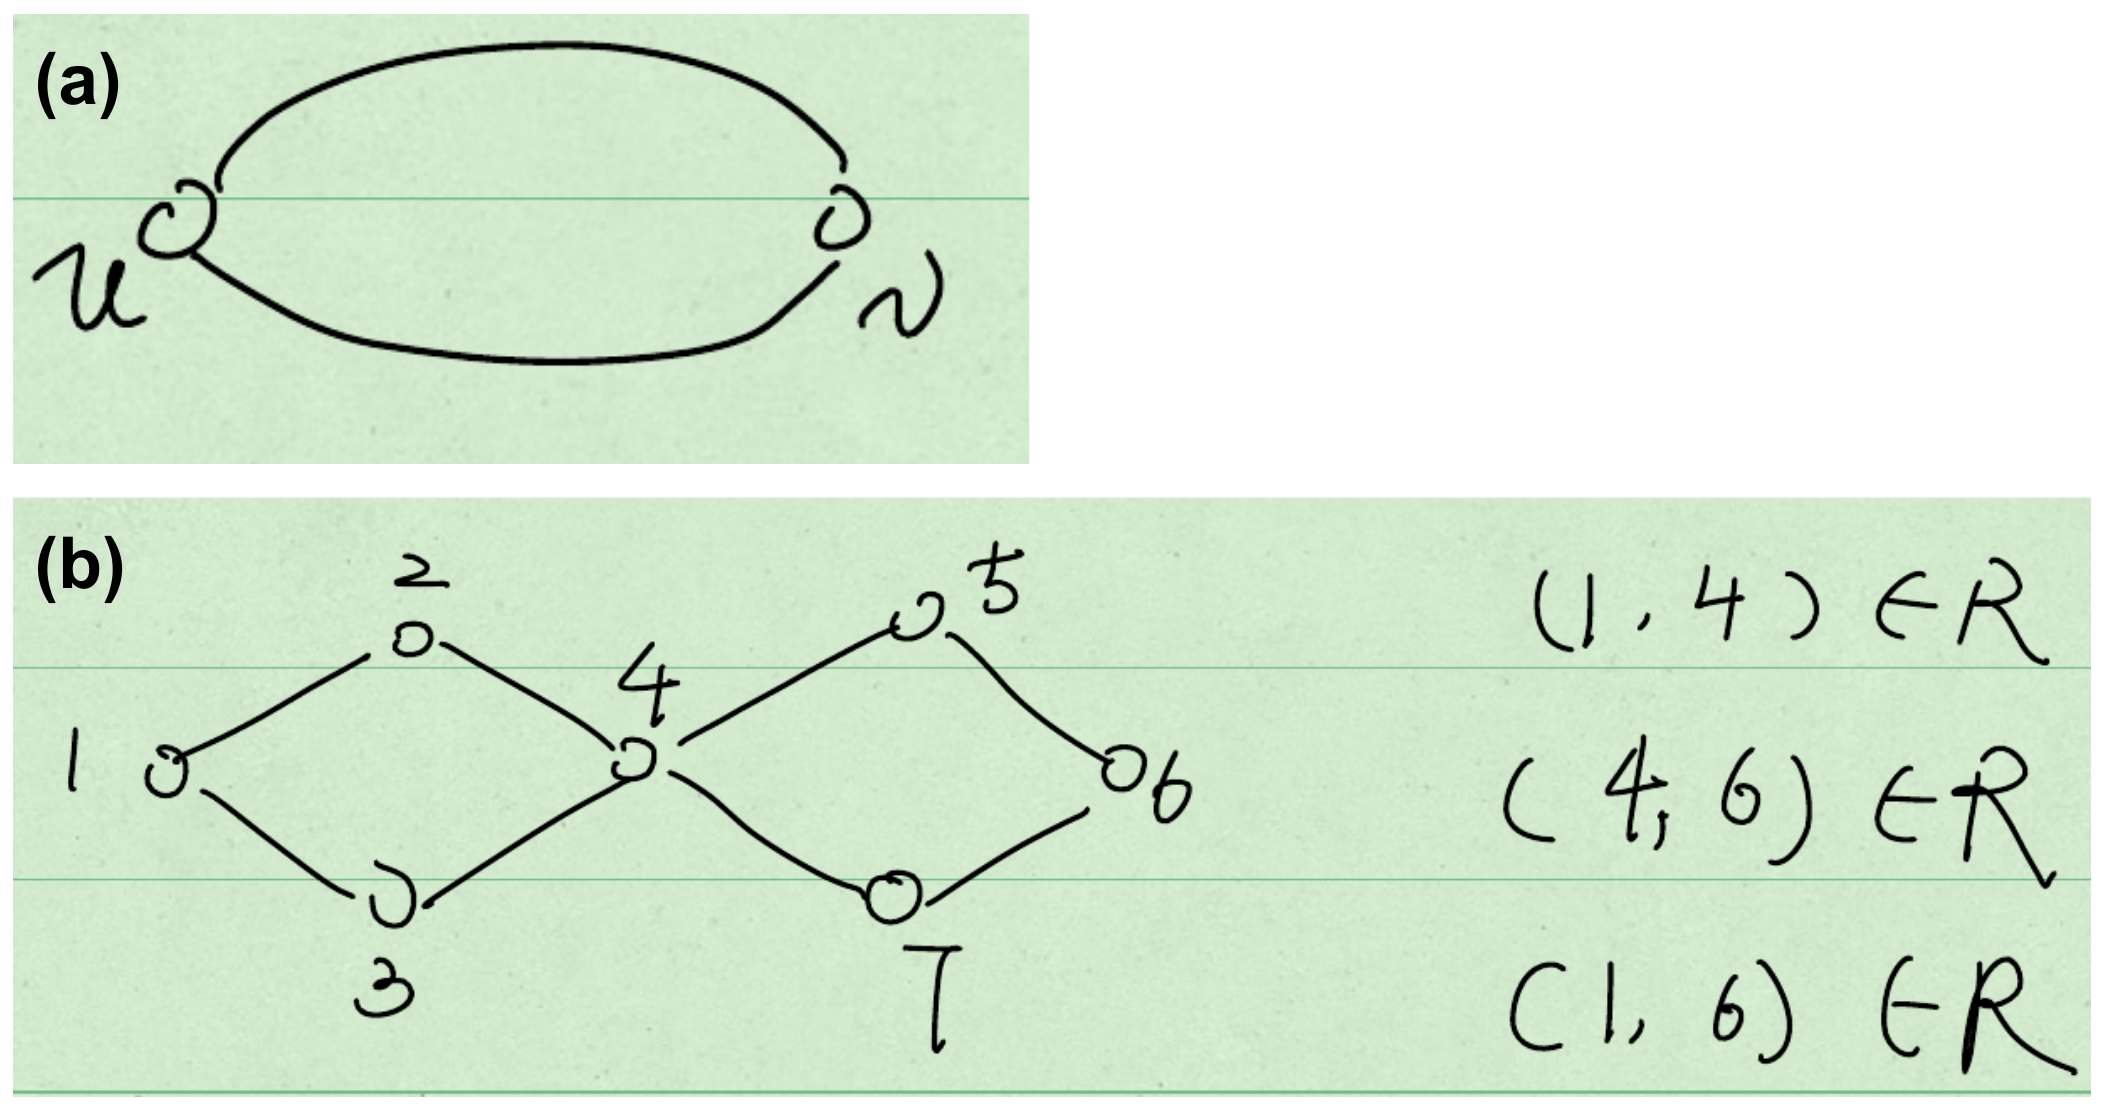
\includegraphics[width=0.5\textwidth]{relation.png}
\end{figure}

\paragraph{The relation $R$ on edges defined as follows:}
\begin{itemize}
\item For any edge $e$, $(e,e) \in R$.
\item If $e_1, e_2$ are two distinct edges, then $(e_1, e_2) \in R$ iff there 
is a simple cycle that passes through $e_1, e_2$.
\end{itemize}

Assume $R$ is an equivalent relation on edges. The property of equivalent 
relation is it divides the set on which it is defined into partitions of 
equivalent class.

Assume $R$ is an equivalence relation on edges. R partitions edges into 
equivalence class $E_1, E_2, \cdots, E_k$. 

For a sanity check, if $k = 1$ then the graph is a bi-connected graph. 
% TODO: ? why
Define component $G_i$ as the graph consist of edges $E_i$ together with a 
vertex set $V_i$ consist of the every point of $E_i$.

A vertex belongs to more than one components iff it is not clean.

\subsection{Find Articulation Points}
Assume $G$ is connected and undirected, start DFS at node $s$, so $s$ is the root of DFS tree.

\subsubsection{Check root of DFS Tree}
\paragraph{Case 1:} Suppose $s$ has one child in DFS tree. In this case, $s$ is 
not an articulation point since the removal of $s$ won't disconnect the graph. 
See example in (a).

\paragraph{Case 2:} Suppose $s$ has more than 1 child in DFS tree. $s$ is 
an articulation point because back edges only go between ancestor and 
descendant. The nodes in subtree $T(v_1)$ and $T(v_2)$ are not ancestor nor 
descendant between each other. Therefore all the paths connecting $T(v_1)$ and $T(v_2)$ must go through $s$. Hence $s$ is an articulation point. See example in (b).

\subsubsection{Check Interior Nodes}

Note that no leaf can be articulation point because moving a leaf the DFS tree is still connected.

Assume $v$ is an internal node and has $k$ leaves. What are the conditions for $v$ to be an articulation point? 
\begin{claim}
 An internal node $v$ is an articulation point \textbf{iff} it has a child $u_i$ such that here is no back edge from the subtree rooted at $u_i$ to a proper ancestor of $v$. See example in (c).
\end{claim}

\begin{figure}[H]
\centering
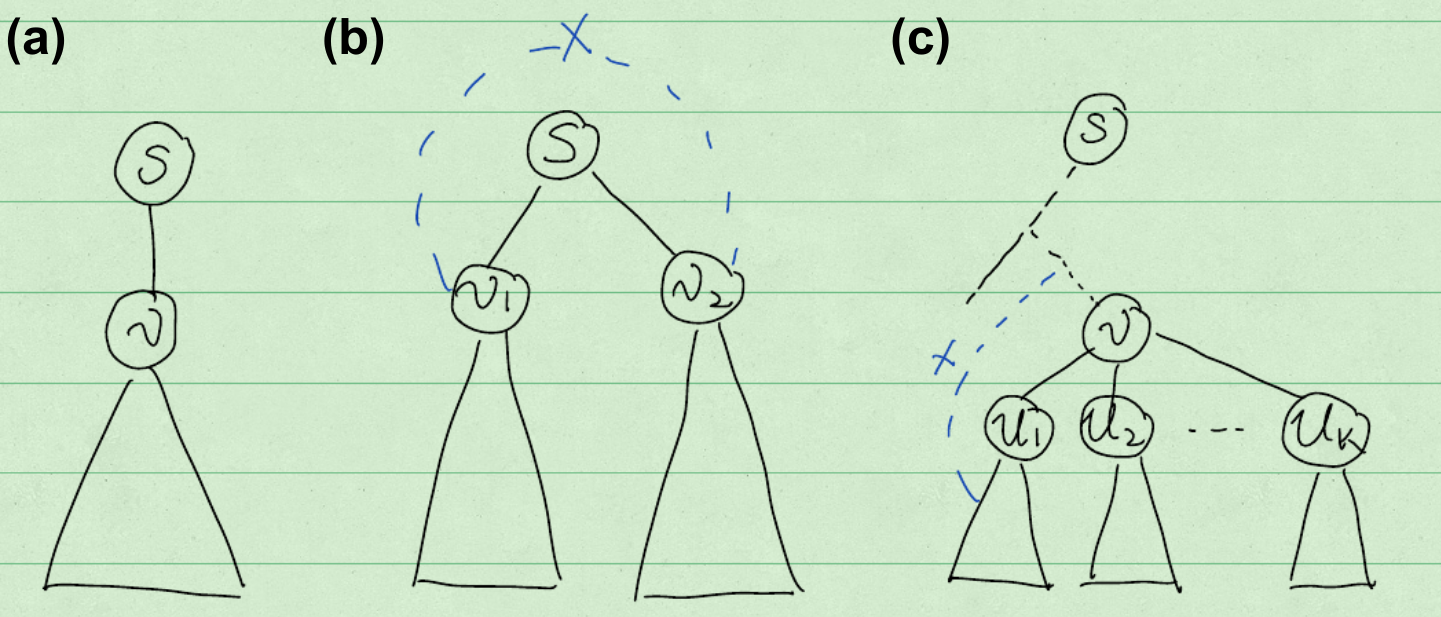
\includegraphics[width=0.8\textwidth]{find-articulation.png}
\end{figure}

\subsection{DFS: Find Bi-connected Components.}
\paragraph{Main idea:} Store visited edges in a stack while DFS on a graph and keep looking for Articulation Points. 
\begin{itemize}
 \item As soon as an Articulation Point $u$ is found, all edges visited while DFS from node $u$ onward will form one biconnected component. 
 \item When DFS completes for one connected component, all edges present in stack will form a biconnected component.
 \item If there is no Articulation Point in graph, then graph is biconnected and so there will be one biconnected component which is the graph itself.
\end{itemize}

\subsubsection{How to check articulation point?}
\begin{claim}
 If $u$ is an ancestor of $v$ in the DFS tree, then $s(u) < s(v)$.
\end{claim}
\paragraph{Note:} smaller number of start time $s$ means higher up of the tree. 

How the algorithm works? What does DFS keep track of? 

We want to know which vertices as we go back out of the subtree could be 
articulation points. The higher a back edge goes, the more vertices are ruled 
out to be articulation points. So \textbf{keep track of the highest back edge 
going out from every subtree}. Hence we are able to find the highest ancestor 
that an edge going through from the subtree. Then we know every vertex along the 
way can not be articulation point because of this subtree. (But still, other 
subtrees may cause them to be an articulation point.)

This is where the postorder comes in. In the example, suppose $x_1$ goes to vertex $p_1$ which is the highest back edge to reach from any where of $T(x_1)$. So the smallest number of start time reached from $T(x_1)$ is $s(p_1)$. From $x_2$ we have some edge goes up to vertex $p_2$, which is the highest back edge to reach from any where of $T(x_2)$.

\begin{figure}[H]
\centering
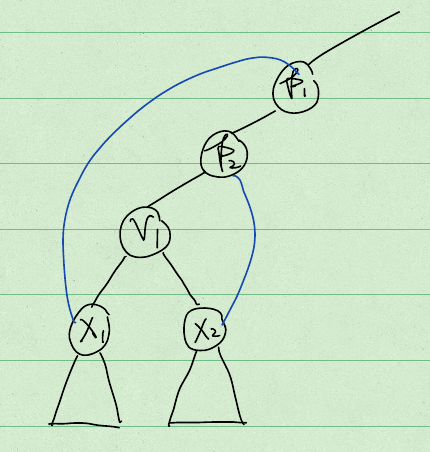
\includegraphics[width=0.3\textwidth]{dfs-claim.png}
\end{figure}

\begin{definition}
 \textbf{low(x)} is the smallest \textbf{start time} of vertices reachable by a back edge from subtree rooted at $x$. 
\end{definition}

Suppose $v$ has just two child $x_1$ and $x_2$,
\[\text{low}(v) = \min (\text{low}(x_1), ~\text{low}(x_2), ~\text{s}(u): (v, u) \text{ is a back edge})\]

What make $v$ an articulation point?
\begin{claim}
 For any node $v$ that is not the root, $v$ is an articulation point \textbf{if 
and only if }
 
 there exist a child $u_i$ of $v$ such that $\text{low}(u_i) \ge s(v)$.
\end{claim}

\paragraph{Notes:} The claim means the child of $v$ will not send any back edge 
to any where above $v$. Sending back edges only to $v$ and below means removing 
$v$ the whole subtree will fall apart.
\subsection{Wrapper of DFS}
DFS is used to search the entire graph. Usually DFS is wrapped by another 
function to traverse all the vertices in the graph.

DepthFirstSearch($G$):\\
\tab \tab While there is an unexplored vertex $x$,\\
\tab \tab \tab dfs($G$, $x$)

\subsubsection{Time}
In this case, we still have start time and finish time continue all the way 
though the outside layer. We start from inner layer of one $s$ and you might 
advance to certain point of time then find out that you have no more vertex to 
visit. So we go back to the outer loop start DFS at some other point and keep 
the time going. So the start time and finish will still between $1$ and $2n$.
\section{Directed Graph}
In directed graph, an edge is an ordered pair. 
\subsection{Edges}
\begin{itemize}
 \item Tree edges: edges where new vertices are discovered.
 \item Back edges: $(3 \rightarrow 1)$
 \item Forward edge $(1 \rightarrow 3)$ could be forward edge if DFS went $(1 
\rightarrow 2 \rightarrow 3)$.
 \item Cross edge
\end{itemize}

\begin{figure}[H]
\centering
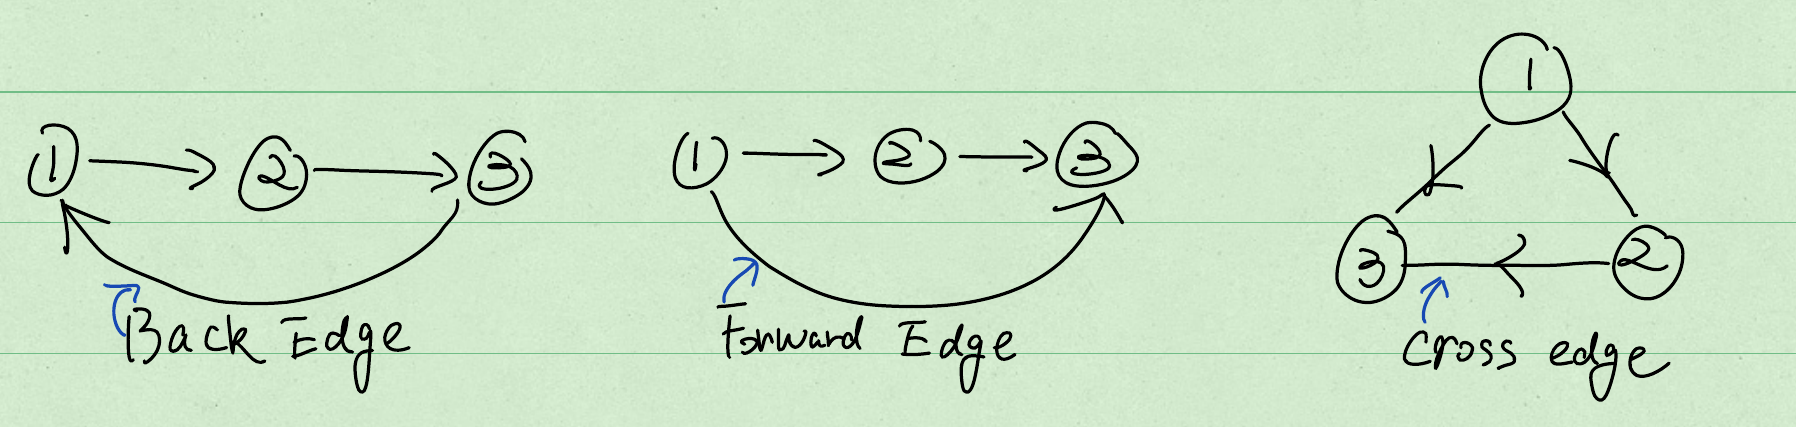
\includegraphics[width=0.45\textwidth]{edges.png}
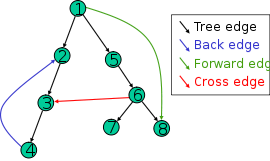
\includegraphics[width=0.3\textwidth]{edges-2.png}
\end{figure}
\begin{claim}
\textbf{Restriction of cross edge:} If $(u, v)$ is a cross edge, then 
$s(u)$ > $s(v)$. In other words, $v$ is discovered before $u$.
\end{claim}
\begin{claimproof}
By contradiction, if $(u, v)$ is a cross edge and $u$ is discovered before $v$, 
we cannot let DFS left $u$ and discover $v$ without go though $(u, v)$. 
Therefore, $v$ will be a child of $u$ instead of a node in other DFS tree.
\end{claimproof}
\subsection{Directed Acyclic Graph (DAG)}
\subsubsection{Maximum Number of edges}
\begin{itemize}
\item How many edges a undirected \textbf{acyclic} graph could have at most? 
$N-1$
\item How many edges a directed \textbf{acyclic} graph could have at most? 
$\frac{N(N-1)}{2}$
\end{itemize}
\subsubsection{Algorithm}
\begin{itemize}
 \item Input: Directed acyclic graph $G$.
 \item Goal: Solve topological sort problem by finding the topological order. 
In other words, find an order of the vertices such that for each edge $(u, v)$, 
$u$ precedes $v$ in order.
\end{itemize}
\begin{theorem}
 Any directed acyclic graph has a topological order.
\end{theorem}

\begin{proof}
Show every DAG has some node with no incoming edges. Then remove the node from 
the graph and get a smaller DAG. Then use induction to prove the theorem is 
true.

\begin{claim}
Every DAG has some node with no incoming edge.
\end{claim}
\begin{claimproof}
Given a graph DAG and reverse the directions of all the edges. Then we want to 
argue that there is no outgoing edge for some nodes in the graph.

For contradiction, suppose the argument is not true and every node has some 
outgoing edge. Then start walking from some vertex $v$ and this walking will 
keep on continuing since every vertex has some outgoing edge. But the graph is 
finite. Continuing walking on a finite graph means there must be cycles in the 
graph. We meet a contradiction since the graph is DAG.
\end{claimproof}
\end{proof}

The first principle algorithm for topological sorting is to track the in-degree 
of every vertex, which is the number of edges come in to the vertex. First 
output the vertex $v$ with in-degree zero. Then go to the adjacency list of $v$ and decrease the in-degree of every neighbor by 1. Remove $v$ from the graph and 
repeat.

Solution based DFS.
\begin{theorem}
 If $G$ is a DAG and $(u, v)$ is an edge, then on any DepthFirstSearch($G$), 
$f(u) \ge f(v)$.
\end{theorem}

\begin{proof}
Prove by cases analysis.
 \begin{itemize}
  \item Case 1: $s(u) < s(v)$. $u$ is discovered before $v$. Then $v$ will 
become a descendant of $u$ (may not be child).
  \item Case 2: $s(u) > s(v)$. $v$ is discovered before $u$. 
  \begin{itemize}
   \item If we discovered $u$ in the course of DFS($v$), then there must be 
a path from $v$ to $u$, which means $G$ has a cycle. 
$\Rightarrow\mskip-\thinmuskip\Leftarrow$
    \item If $u$ is not in the subtree of $v$ as the following example, 
then obviously $f(v) < f(u)$.
        \begin{figure}[H]
        \centering
        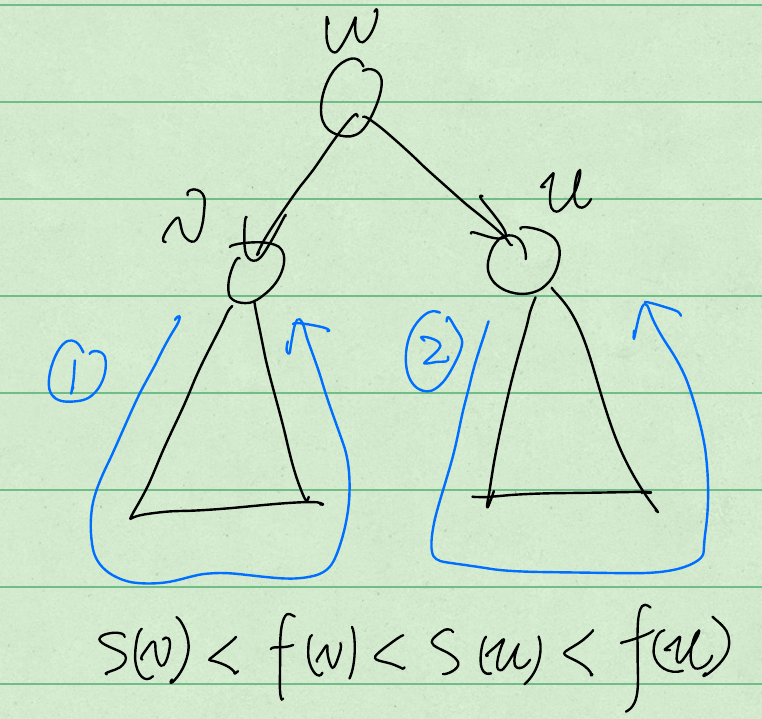
\includegraphics[width=0.3\textwidth]{dfs-s-f.png}
        \end{figure}
  \end{itemize}
 \end{itemize}
\end{proof}

So, \[s(v) < f(v) < s(u) < f(u)\]
Therefore the algorithm should be:

TopologicalSort($G$):\\
\tab\tab DepthFirstSearch($G$):\\
\tab\tab\tab\tab Output vertices in reverse order of finish time.

\subsection{Strongly Connected Graph}

\subsubsection{Basics}
Give a directed graph $G = (V, E)$, what is the correct connectivity relation?

We want the relation to be equivalent. The edge between two nodes is not 
symmetric relation in directed graph. Therefore we create a equivalent relation 
by setting symmetric in the definition.

\begin{definition}
 $R = \{(u, v): \text{There are paths from $u$ to $v$ and from $v$ to $u$}\}$
\end{definition}

$R$ is reflective, symmetric and transitive. So $R$ is an equivalent relation 
on the vertices.

\begin{definition}
$R$ partitions $V$ onto $V_1,~V_2,~\cdots, V_k$. (Equivalence Classes)

If $V_1 \subset V$, which is the vertex set of $G = (V, E)$, it induces the 
sub-graphs
\[G_{V_i} = (V_i, ~E \cap (V_i \times V_i) )\]
For simplicity, call $G_{V_i}$ as $G_i$. $G_i$'s are \textbf{the 
strongly connected components} of $G$.
\end{definition}


It is possible to have edges connecting different strongly connected 
components. See example as follows.
\begin{figure}[H]
\centering
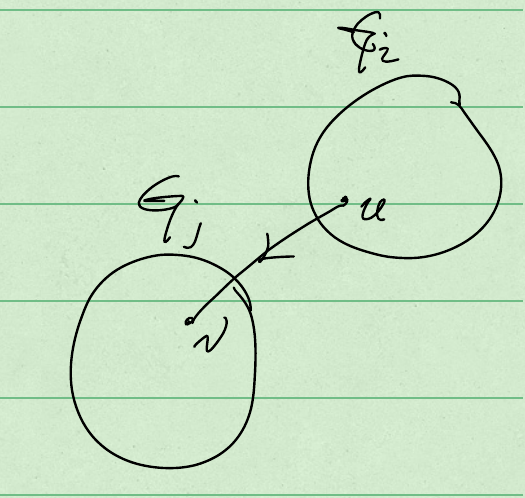
\includegraphics[width=0.2\textwidth]{edge-strongly-connected-components.png}
\end{figure}

\begin{definition}
 The \textbf{strongly connected graph} of directed graph $G(V, E)$ is 
$G_{SCC}(V_{SCC}, E_{SCC})$, where
\begin{itemize}
 \item $V_{SCC} = \{c_i: G_i \text{ is a strongly connected components}\}$.
 \item $E_{SCC} = \{(c_i, c_j): \exists v_i \in G_i \text{ and }v_j \in G_j, 
~(v_i, v_j) \in E \}$
\end{itemize}
\end{definition}
Here $G_{SCC}$ is actually a quotient graph.

Example, $(a)$ in the following plot is the Graph $G$ and $(b)$ is the strongly 
connected graph of $G$. The equivalence class of $G$ is $\{\{1, 2, 3, 4\}, 
\{3, 6, 7\}\}$.

\begin{figure}[H]
\centering
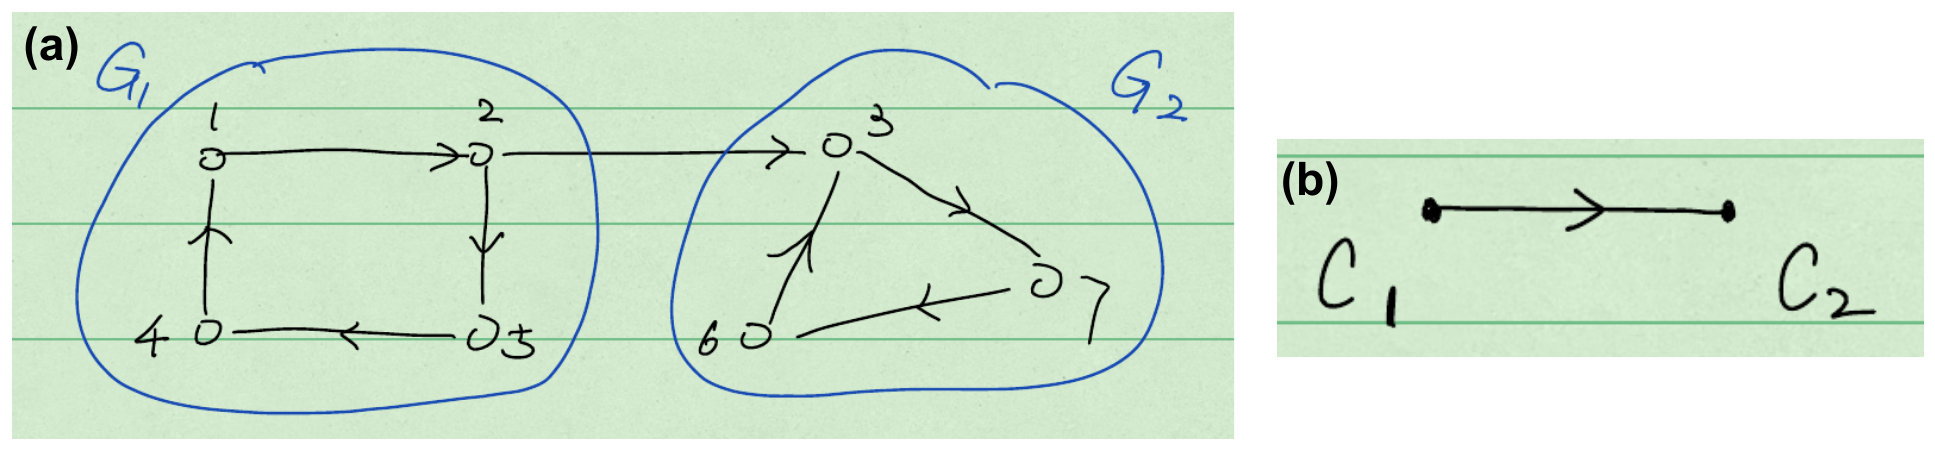
\includegraphics[width=0.7\textwidth]{scg.png}
\end{figure}

\begin{theorem}
 $G_{SCC}$ is acyclic.
\end{theorem}

\begin{proof}
 The components we have found are the maximal with respect to the relation on 
both side to reach other. Prove the theorem by contradiction. Suppose we have a 
cycle as the following plot. Because there must be a path from $u$ to $v$ and 
vice versa. Then , we are able to merging $G_1$, $G_3$. In fact, all three 
components can be merged together.

\begin{figure}[H]
\centering
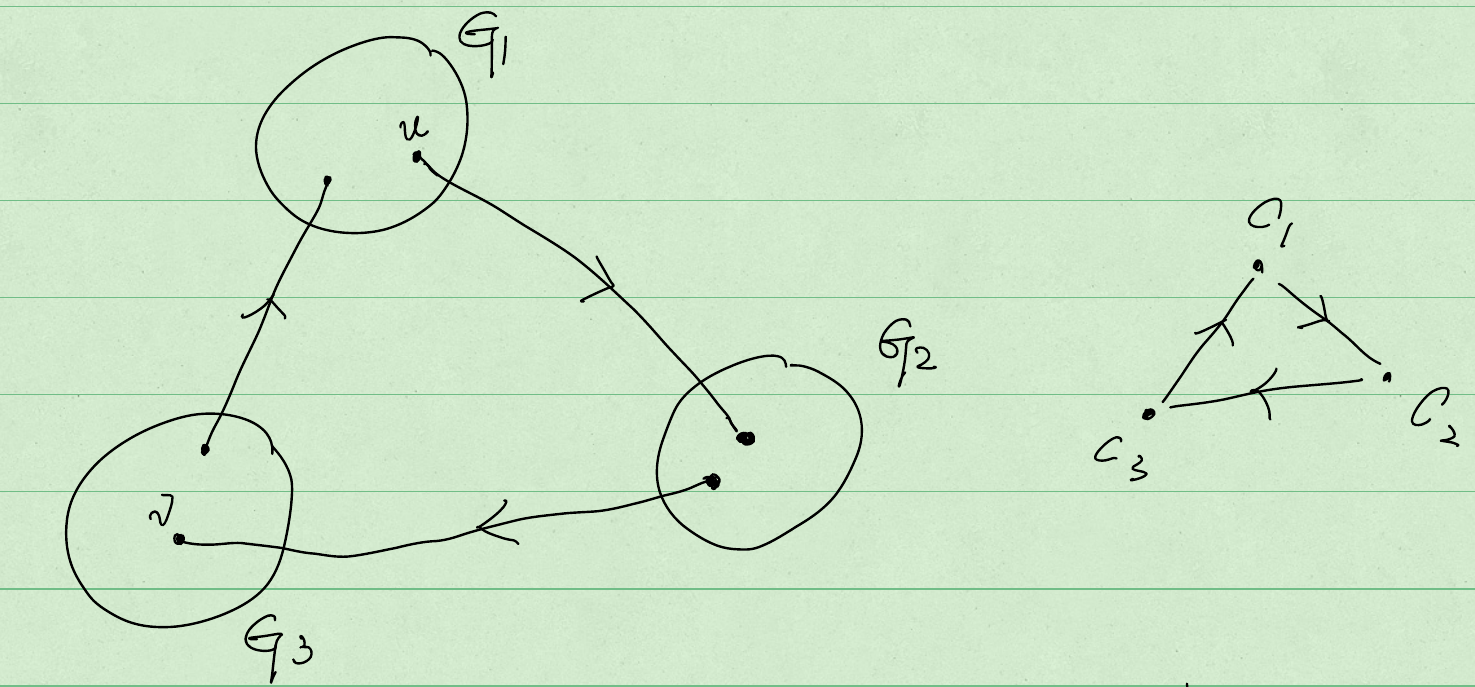
\includegraphics[width=0.45\textwidth]{scg-contradiction.png}
\end{figure}
\end{proof}

Many algorithm on directed graph works on first decomposing the graph into 
strongly connected components.

DFS decomposes a directed graph into SCC's.

\subsubsection{Finish Time}
Now we first gave a \textbf{false theorem} and make it right.
\begin{theorem}\textbf{[False Theorem]}

Suppose $G$ is an arbitrary graph and $G_{SCC}$ is a DAG. If $c_i, ~c_2 \in V_{SCC}$ are nodes corresponding to two SCC's $G_1$ and $G_2$ in $G$ and $(c_i, ~c_2) \in E_{SCC}$, then in DFS($G$), every vertex in $G_1$ finish after every vertex in $G_2$. 
\end{theorem}

\begin{proof}
 Prove the theorem is false by a counter example as follows:
\begin{figure}[H]
\centering
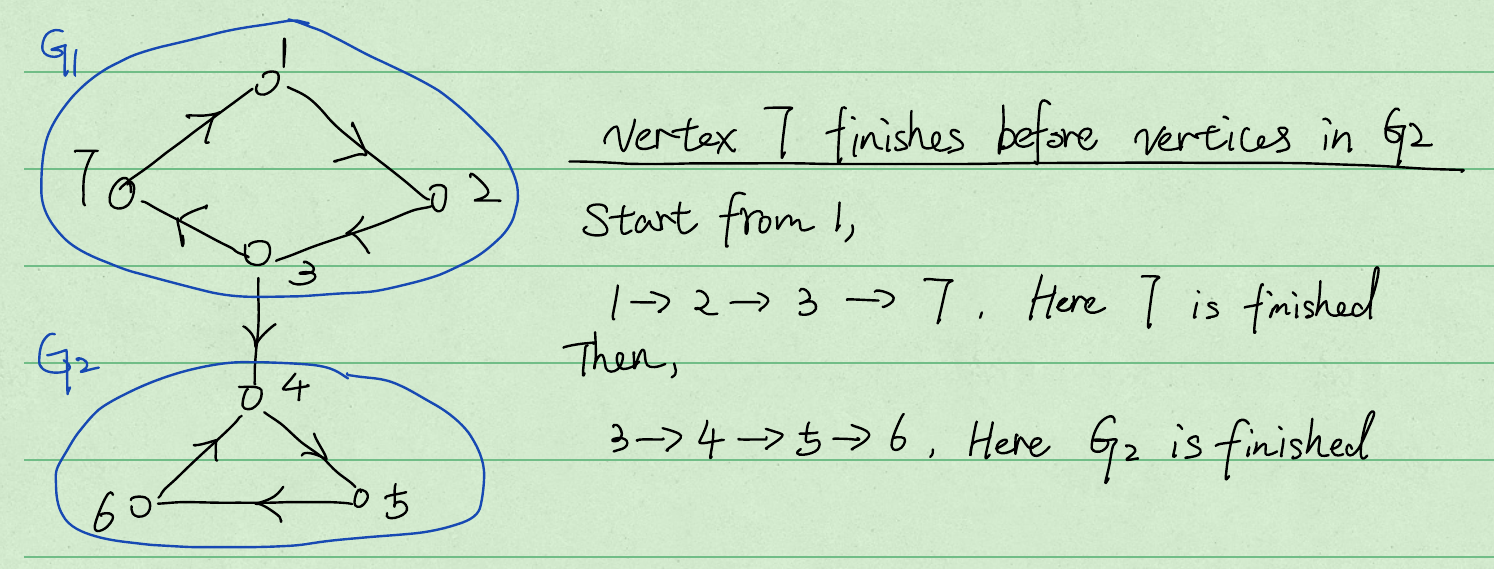
\includegraphics[width=0.7\textwidth]{scc-finish-time.png}
\end{figure}
\end{proof}

\begin{theorem}\textbf{[Updated Theorem]}

Suppose $G$ is an arbitrary graph and $G_{SCC}$ is a DAG. If $c_i, ~c_2 \in V_{SCC}$ are nodes corresponding to two SCC's $G_1$ and $G_2$ in $G$ and $(c_i, ~c_2) \in E_{SCC}$, then in DFS($G$), \textbf{there exist a vertex} in $G_1$ finish after every vertex in $G_2$. 
\end{theorem}

\begin{proof}
 TODO: Read the proof in the book.
\end{proof}

\subsubsection{Kosaraju's Algorithm}
\begin{definition}
$G_{SCC}$ is a DAG. So, $G_{SCC}$ has one or more vertices with no in-coming 
edges. These vertices are called \textbf{sources}.
\end{definition}

\begin{claim}{}
If $v$ is the vertex with largest $f(v)$ in a DFS($G$). Then $v$ must lies in 
the source component. 
\end{claim}

\begin{claimproof}{}
Prove by contradiction.

If $v$ does not lie in the source component but in some other component $C$. So 
$v$ must have some in-coming edge to make it not a source. That means that 
some vertex $u$ must finish later than everything in the component $C$ because 
of the theorem of finishing time. Therefore $v$ could not be the latest 
finishing vertex.
\begin{figure}[H]
\centering
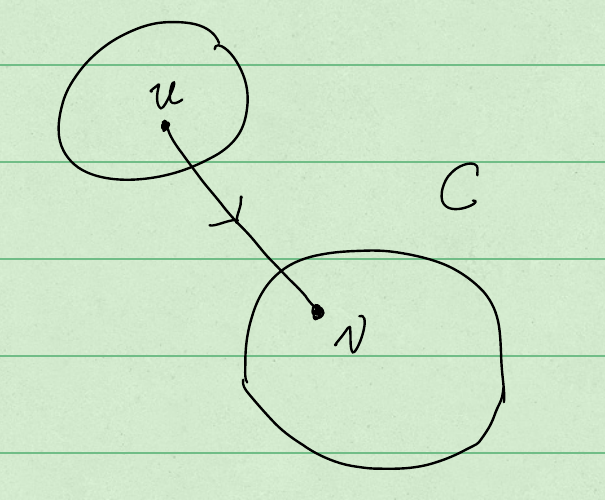
\includegraphics[width=0.3\textwidth]{source-finish-time.png}
\end{figure}
\end{claimproof}


\paragraph{Kosaraju Algorithm}
\begin{itemize}
 \item One DFS(G) to record the nodes of finish times. Let $f_1(v)$ be the 
finish time of $v$ in this DFS.
\item Reverse all the edges in $G$ to create the graph $G^R$.
\item Do DFS($G^R$) with one constrain:
    \begin{itemize}
    \item In the outer procedure, always choose the undiscovered vertex $v$ 
with the greatest $f(v)$.
    \end{itemize}
\end{itemize}

\paragraph{Notes}
\begin{itemize}
 \item The vertex $v$ with greatest $f_1(v)$ lies in a sink component of $G^R$.
\item $G$ and $G^R$ have the same strongest connected component DFS($G^R$) start 
at $v$ will only discover the SCC containing $v$.
\item When the inner call to DFS($G^R, ~v$) finishes, output all the discovered 
vertices as one SCC of $G$.
\item When we return to the outer loop and pick the undiscovered vertex with 
the greatest finish time, we know inductively that we will find all SCC's.
\end{itemize}

\begin{figure}[H]
\centering
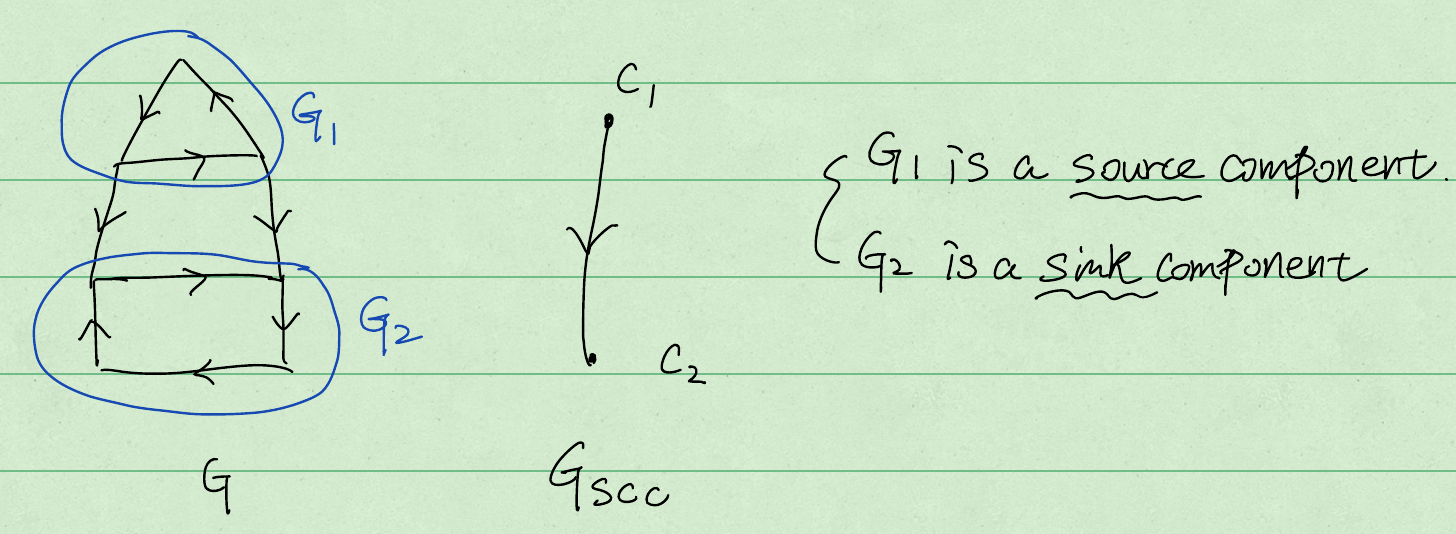
\includegraphics[width=0.6\textwidth]{scc-source-sink.png}
\end{figure}

\paragraph{Running Time}
Two DFS's and reverse the edges in the graph. All the steps are linear. So 
this is a $O(m + n)$ algorithm. $m, n$ are the numbers of vertices and edges.
\end{document}
